Il periodo di Analisi ha inizio con la formazione dei gruppi e termina con la consegna dei documenti per la RR. \newline
Ogni attività da svolgere in questa fase corrisponde alla stesura di uno dei documenti seguenti: 
\begin{itemize}
	\item \textbf{Norme di progetto:}
	documento redatto dall'Amministratore nel quale sono presenti le norme di collaborazione fra i membri del gruppo \gruppo ;
	\item \textbf{Studio di fattibilità:}
	documento redatto dagli Analisti nel quale è presente un'analisi di massima di tutti 	i capitolati, basandosi sulla quale il gruppo sceglie il capitolato per cui presentare un'offerta;
	\item \textbf{Analisi dei Requisiti:}
	documento redatto dagli Analisti nel quale è presente un'analisi più approfondita del capitolato scelto;
	\item \textbf{Piano di progetto:}
	documento redatto dal \Res \space nel quale sono pianificati lo svolgimento del progetto e l'utilizzo delle risorse;
	\item \textbf{Piano di qualifica:}
	documento redatto dagli Analisti nel quale è presente la strategia del gruppo \gruppo \space per garantire la qualità del progetto;
	\item \textbf{Glossario:}
	documento nel quale sono presenti le definizioni di alcuni dei termini presenti nei precedenti documenti, allo scopo di disambiguarne il significato;
	\item \textbf{Lettera di presentazione:}
	lettera nella quale il gruppo \gruppo \space si candida ufficialmente come fornitore per il capitolato scelto.
\end{itemize}

\begin{figure}[H]
	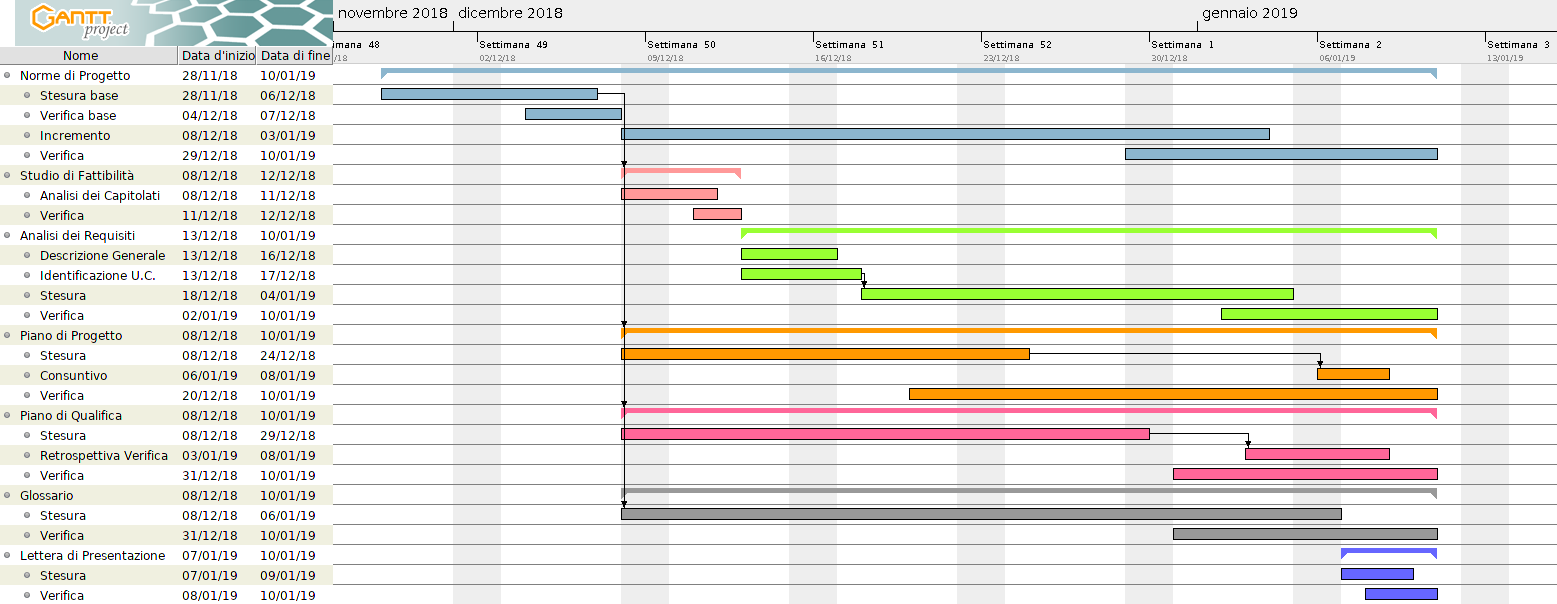
\includegraphics[width=1\linewidth]{Pianificazione/Analisi_Gantt.png}
	\caption{Diagramma di Gantt del periodo di Analisi}
\end{figure}
